
% This LaTeX was auto-generated from an M-file by MATLAB.
% To make changes, update the M-file and republish this document.

\documentclass{article}
\usepackage{graphicx}
\usepackage{color}

\sloppy
\definecolor{lightgray}{gray}{0.5}
\setlength{\parindent}{0pt}

\begin{document}

    
    
\subsection*{Contents}

\begin{itemize}
\setlength{\itemsep}{-1ex}
   \item Exercise1
\end{itemize}
\begin{verbatim}
function x = Exercise1( L, A, b, M )
\end{verbatim}


\subsection*{Exercise1}

\begin{par}
Generate a periodic, truncated, decaying exponential function: L - Total number of samples in the waveform A - Beginning amplitude of the exponential function b - Decay rate of the exponential function M - Number of samples each period will last The function takes the form $A*\exp{-bn}$ Test Paramters: L = 80 A = 2 b = 0.08 M = 20
\end{par} \vspace{1em}
\begin{verbatim}
x = A*exp(-b * mod([0:L-1],M));
\end{verbatim}
\begin{verbatim}
end
\end{verbatim}

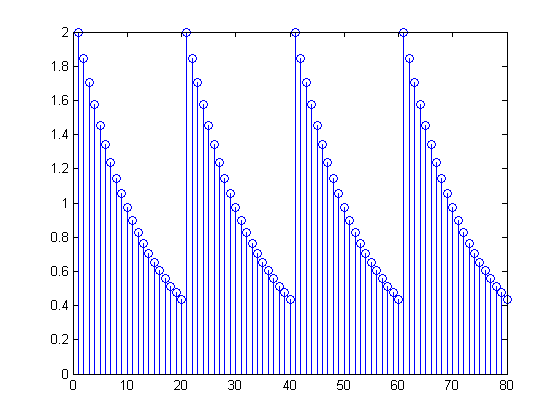
\includegraphics [width=4in]{Exercise1_01.png}



\end{document}
    
